\documentclass[12pt, fleqn, oneside]{book}
\usepackage{graphicx}
\usepackage{amssymb}
\usepackage{multicol}
\usepackage{amsmath}
\usepackage{ifthen}
\usepackage[margin=.75in,bindingoffset=.5in]{geometry}
\usepackage{color}
\usepackage{setspace}
\usepackage{multicol}

\usepackage{fancyhdr}
% \fancyhead[CE,CO]{\raisebox{-.05in}{\rule{6.5in}{.01in}}}
% \let\origheadrule\headrule
\fancyhead[CO]{\raisebox{-.05in}{\rule{6.5in}{.01in}}}
\fancyhead[LE,LO]{}
\fancyhead[RO]{{\footnotesize \textsl{\thepage}}  }
\fancyhead[Re]{  }
\fancyfoot[CE, CO]{}
\renewcommand{\headrulewidth}{2pt}
% \def\headrule{%
  % \ifodd\value{page}\origheadrule\else\relax\fi}
\def\chaptermark{}

\begin{document}
\setcounter{page}{51}

\setlength{\parindent}{0in}

\pagestyle{empty}

\centerline{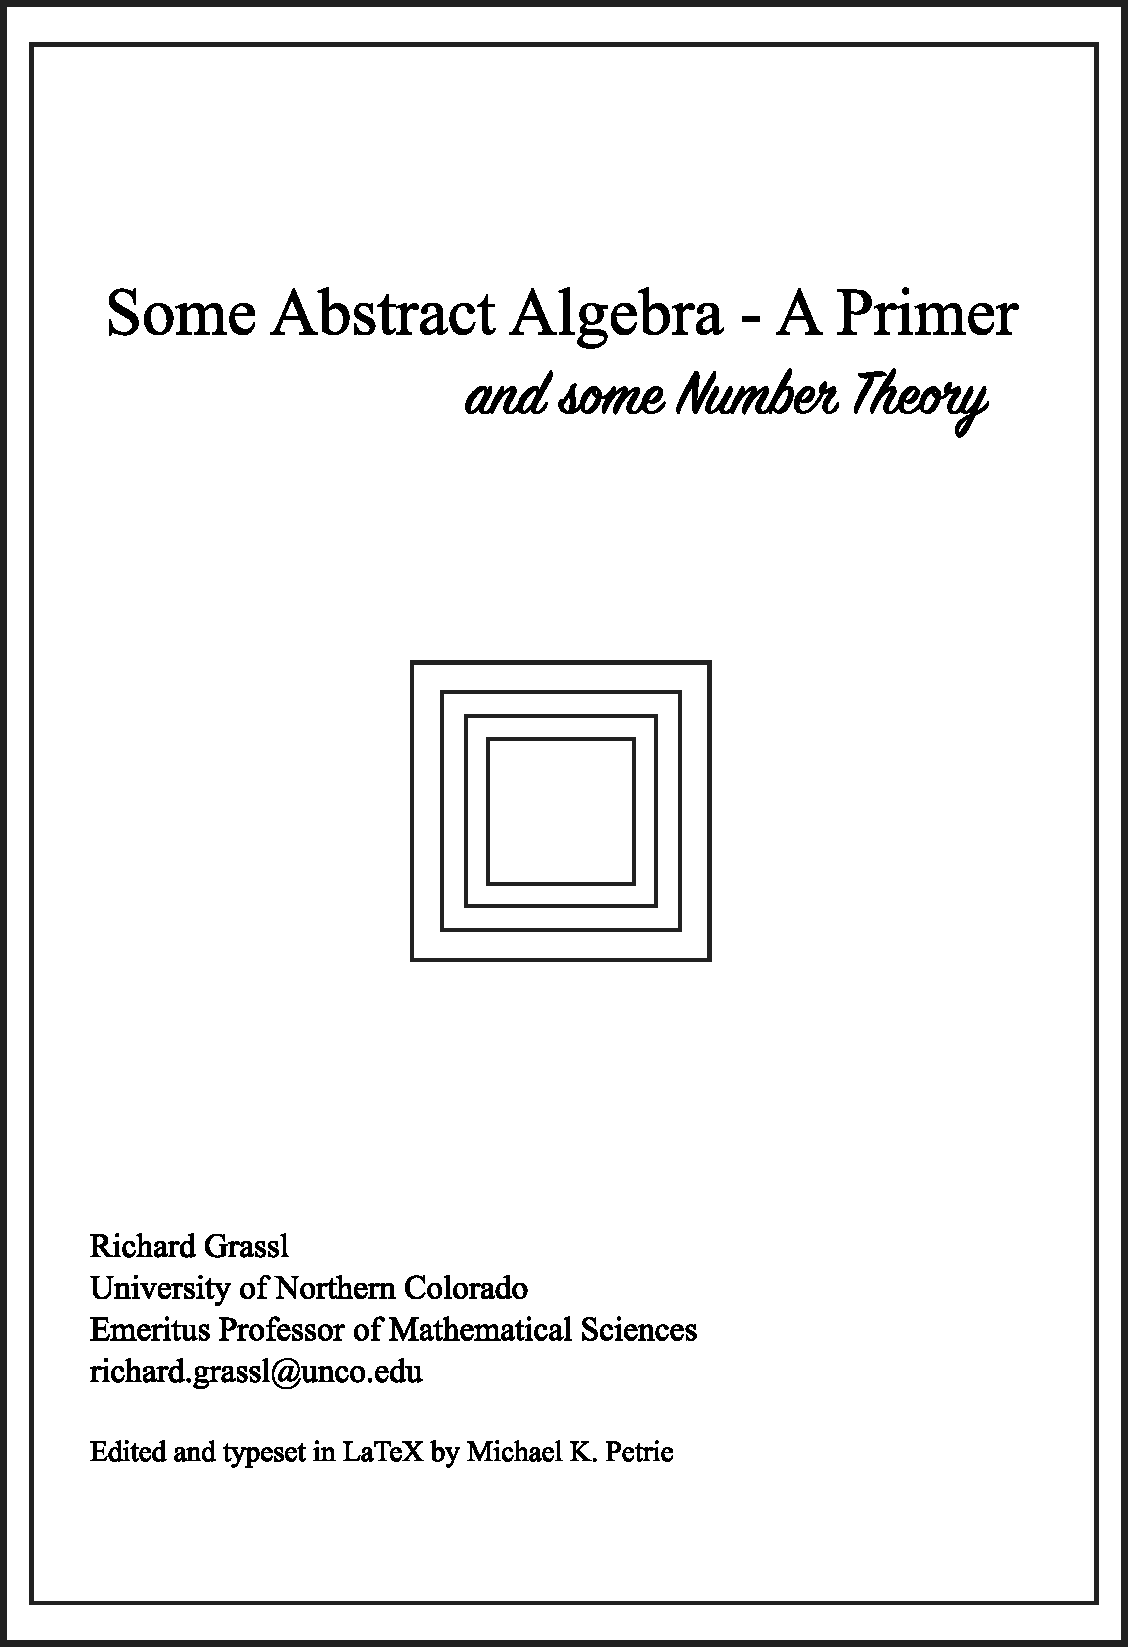
\includegraphics[width=6in]{Coverpage.pdf}}
~
\clearpage

\thispagestyle{plain}
\tableofcontents

\cleardoublepage

\pagestyle{fancy}

% \pagenumbering{roman}
%{\Large{Contents}}\\[.2in]
%\begin{minipage}[b]{3in}
%\begin{tabular}{lr}
%Three Tables \dotfill & 1\\
%Closure \dotfill & 2\\
%Residue Classes \dotfill & 6\\
%Modular Arithmetic \dotfill & 7\\
%Cancellation \dotfill & 9\\
%Permutations \dotfill & 10\\
%Subgroups \dotfill & 12\\
%Order \dotfill & 13\\
%Group Tables \dotfill & 14\\
%Complex Numbers \dotfill & 15\\
%Table of Roots \dotfill & 17\\
%Sixth Roots of Unity \dotfill & 18\\
%Eighth Roots of Unity \dotfill & 19\\
%Composition of Functions \dotfill & 20\\
%Euler $\phi$-Function \dotfill & 22\\
%Invertibles \dotfill & 24\\
%Preservation of Operation \dotfill & 25
%\end{tabular}
%\end{minipage}
%\begin{minipage}[t]{4in}
%\begin{tabular}{lr}
%A Special Isomorphism \dotfill & 26\\
%Matching Groups \dotfill & 27\\
%Groups of Order 8 \dotfill & 28\\
%Five Groups of Order 8 \dotfill & 33\\
%Group Tables, Isomorphisms \dotfill & 34\\
%Fundamental Theorem \dotfill & 35\\
%Which Direct Product \dotfill & 37\\
%Rings, But Not I.D. \dotfill & 38\\
%Polynomials in $Z_n[x]$ \dotfill & 39\\
%Another Ring \dotfill & 41\\
%Summary of Rings \dotfill & 42\\
%A Field With 9 Elements \dotfill & 43\\
%Application of a Famous Theorem \dotfill & 44
%\end{tabular}
%\end{minipage}
%
%
%
%
% \thispagestyle{empty}
% \phantom{.}
% \vfill
% \centerline{\Large \bf{Contents}}
% \rule{0in}{.4in}\\
% \begin{tabular}{lr@{\hspace{.6in}}lr}
% \phantom{Composition of Functions......}&{\underline {Page}} &\phantom{Application of a Famous Theorem.....}& \underline{Page}\\[.2in]
% Three Tables \dotfill & 1 &  Invertibles \dotfill & 24 \\[.1in]
% Closure \dotfill & 2 & Preservation of Operation \dotfill & 25 \\[.1in]
% Residue Classes \dotfill & 6& A Special Isomorphism \dotfill & 26 \\[.1in]
% Modular Arithmetic \dotfill & 7& Matching Groups \dotfill & 27 \\[.1in]
% Cancellation \dotfill & 9 & Groups of Order 8 \dotfill & 28 \\[.1in]
% Permutations \dotfill & 10 & Five Groups of Order 8 \dotfill & 33 \\[.1in]
% Subgroups \dotfill & 12 & Group Tables, Isomorphisms \dotfill & 34 \\[.1in]
% Order \dotfill & 13& Fundamental Theorem \dotfill & 35 \\[.1in]
% Group Tables \dotfill & 14& Which Direct Product \dotfill & 37 \\[.1in]
% Complex Numbers \dotfill & 15 & Rings, But Not I.D. \dotfill & 38\\[.1in]
% Table of Roots \dotfill & 17 & Polynomials in $Z_n[x]$ \dotfill & 39\\[.1in]
% Sixth Roots of Unity \dotfill & 18 & Another Ring \dotfill & 41 \\[.1in]
% Eighth Roots of Unity \dotfill & 19& Summary of Rings \dotfill & 42 \\[.1in]
% Composition of Functions \dotfill & 20& A Field With 9 Elements \dotfill & 43\\[.1in]
% Euler $\phi$ - Function \dotfill & 22& Application of a Famous Theorem \dotfill & 44\\[.1in]
% \end{tabular}
% \vfill\vfill


% \pagenumbering{arabic}
{\large \bf DAY 1  PROPERTIES OF THREE TABLES}\\[.25in]
\addcontentsline{toc}{subsection}{Three Tables}
%
%
%
$\bullet $ = usual complex multiplication\\
\begin{minipage}{2.75in}
$$\begin{array}{c|cccc}
\bullet & \phantom{--}1\phantom{--} & -1& \phantom{--}i &\phantom{--} -i\\
\hline
\\
1&&&&\\
\\
-1&&&&\\
\\
i&&&&\\
\\
-i&&&&
\end{array}$$
\end{minipage}\rule{.75in}{0in}
\begin{minipage}{3in}
{\bf PROPERTIES, OBSERVATIONS}\\
1.\\[.3in]
2.\\[.3in]
3.\\
\end{minipage}\\[.75in]
%
%
%
$\otimes $ = units digit in regular multiplication\\
\begin{minipage}{2.6in}
$$\begin{array}{c|cccc}
\otimes & \phantom{--}1\phantom{--} & 3 & \phantom{--}7 &\phantom{--} 9\\
\hline
\\
1&&&&\\
\\
3&&&&\\
\\
7&&&&\\
\\
9&&&&
\end{array}$$
\end{minipage}\rule{.85in}{0in}
\begin{minipage}{3in}
1.\\[.3in]
2.\\[.3in]
3.\\
\end{minipage}\\[.75in]
%
%
%
$\oplus $ = bitwise addition, 0 if same, 1 if different\\
\begin{minipage}{2.75in}
$$\begin{array}{c|cccc}
\oplus & \phantom{--}00\phantom{--} & 01 & \phantom{--}10 &\phantom{--} 11\\
\hline
\\
00&&&&\\
\\
01&&&&\\
\\
10&&&&\\
\\
11&&&&
\end{array}$$
\end{minipage}\rule{.75in}{0in}
\begin{minipage}{3in}
1.\\[.3in]
2.\\[.3in]
3.\\
\end{minipage}
%
%
%

\clearpage
%
%
%
{\large \bf WORKSHEET ON CLOSURE I}\\[.25in]
\addcontentsline{toc}{subsection}{Closure}
\

\qquad A set $S=\{a,b,c,\dots\}$ is closed under a binary operation $\circ$ if whenever $x$ and $y$ are elements of $S$ so is $x\,\circ\,y$.

\qquad For each of the following if the answer is yes, give a reason and if no, provide a counterexample.\\[.25in]
\underline{\bf{Task 1}} Is $E=\{0,2,4,6,8,\dots\}$ closed under the binary operation of addition?\\ [.2in]
{\Huge $\square$} yes, {\Huge$\square$} no \qquad Reason:  Let $2m$ and $2n$ be arbitrary elements in $E$.\\[.15in]
Then since $\dots$\\[1.25in]
How about under multiplication?\\[1.25in]
\underline{\bf{Task 2}} Is $A=\{0,1,4,9,16,\dots\}$ closed under addition?\\[1.25in]
Under subtraction?\\[1.25in]
Under multiplication?%
%
\clearpage%
%
\underline{\bf{Task 3}} Is the set of all rational numbers of the form $2^m3^n$, where $m,n \in Z$, closed under multiplication?\\[1.5in]
\underline{\bf{Task 4}} Is the set of all positive rational numbers closed under addition?  Multiplication?\\[1.5in]
\underline{\bf{Task 5}} Are the complex numbers of the form $m+ni$ where $m$ and $n$ are integers closed under multiplication?\\[1.5in]
\underline{\bf{Task 6}} Is the set $\{m+n\sqrt{2}: m, n\in Z\}$ closed under multiplication?\\[1.5in]
\underline{\bf{Task 7}} Are the irrationals closed under multiplication? Under subtraction?
%
%
%
\clearpage%
%
%
%
{\large \bf WORKSHEET ON CLOSURE II}\\[.25in]
Let $Z=\{\dots, -2, -1, 0, 1, 2, \dots\}$\\
QUESTION: Which of the sets $3Z,\, 1+3Z,\,2+3Z$ are closed under subtraction?\\[.25in]
\underline{\bf{Task 1}} List the elements of $3Z$; choose two and subtract them.\\[1.25in]
\underline{\bf{Task 2}} What does it mean to say $3Z$ is closed under subtraction?\\[1.25in]
\underline{\bf{Task 3}} Is $3Z$ closed under subtraction?  If yes, prove it.\\[1.25in]
\underline{\bf{Task 4}} Is $1+3Z$ closed under subtraction?\\[1.25in]
\underline{\bf{Task 5}} Is $2+3Z$ closed under subtraction?\\[1.25in]
\underline{\bf{Task 6}} Why must a set of integers contain $0$ to be closed under subtraction?
%
%
%
\clearpage%
%
%
%
{\large \bf WORKSHEET ON CLOSURE III}\\[.25in]
PROBLEM: Prove that if $S$ and $T$ are sets of integers closed under subtraction so is the intersection $S\cap T$.\\[.25in]
\underline{\bf{Task 1}} Say in your own words what it means to say $S$ is closed under subtraction.\\[1.75in]
\underline{\bf{Task 2}} What do you have to show in order to check that $S\cap T$ is closed under subtraction?\\[1.75in]
\underline{\bf{Task 3}} Draw a Venn diagram as an aid, and resolve the problem.\\[1.75in]
\underline{\bf{Task 4}} If $S$ and $T$ are sets of integers closed under subtraction is the union $S\cup T$ also closed under subtraction?  If yes, prove it, if no give a counterexample.
%
%
%
\clearpage%
%
%
%
{\large \bf WORKSHEET ON RESIDUE CLASSES}\\[.25in]
\addcontentsline{toc}{subsection}{Residue Classes}
Congruence Modulo $m$ is an \underline{EQUIVALENCE RELATION} on $Z$, the set of all integers.\\[.25in]
\begin{tabular}{l@{\hspace{.05in}}l}
R &$-$ REFLEXIVE: $a\equiv a(m)$\\
S &$-$ SYMMETRIC: If $a\equiv b(m)$ then $b\equiv a(m)$\\
T &$-$ TRANSITIVE: $a\equiv b(m)$ and $b\equiv c(m)$ then $a\equiv c(m)$
\end{tabular}\\[.25in]
The relation \textit{congruence} partitions $Z$ into disjoint \underline{EQUIVALENCE CLASSES} or \\
\underline{RESIDUE CLASSES}.\\[.25in]
When $m=2$, $Z$ is partitioned into the classes $2Z$ and $1+2Z$.
\begin{equation*}\begin{split}
2Z &= \{\dots, -4, -2, 0, 2, 4, \dots\}\\
1+2Z &= \{\dots, -3, -1, 1, 3, 5, 7, \dots\}
\end{split}\end{equation*}\\[.2in]
\underline{\bf{Task 1}} Explain why the classes $2Z$ and $1+2Z$ are disjoint.\\[2in]
\underline{\bf{Task 2}} What the residue classes when $m=3$?  Are they disjoint?  Why?\\[1.5in]
\underline{\bf{Task 3}}  When $m=4$?  Explain.
%
%
%
\clearpage%
%
%
%
{\large \bf WORKSHEET ON MODULAR ARITHMETIC}\\[.25in]
\addcontentsline{toc}{subsection}{Modular Arithmetic}
$a\equiv b(\text{mod }m)$ means $a$ and $b$ have the same remainder when divided by $m$; or that $a-b$ is divisible by $m$, or $a-b=mk$.  An example: $17\equiv 9(\text{mod } 4)$ since 4 divides $17-9$.\\[.25in]
\underline{\bf{Task 1}} Complete the missing four rows:
$$\begin{array}{c|ccccccccccccc}
&\phantom{-}0&\phantom{-}1&\phantom{-}2&\phantom{-}3&\phantom{-}4&\phantom{-}5&\phantom{-}6&\phantom{-}7&\phantom{-}8&\phantom{-}9&\phantom{-}10&\phantom{-}11&\phantom{-}12\\
\hline\\[-.1in]
\text{Mod } 2&&&&&&&&&&&&&\\
\\
\text{Mod } 3&\phantom{-}0&\phantom{-}1&\phantom{-}2&\phantom{-}0&\phantom{-}1&\phantom{-}2&\phantom{-}0&\phantom{-}1&\phantom{-}2&\phantom{-}0&\phantom{-}1&\phantom{-}2&\phantom{-}0\\
\\
\text{Mod } 4&\\
\\
\text{Mod } 5&\\
\\
\text{Mod } 6&
\end{array}$$\\[1.5in]
\underline{\bf{Task 2}} Tables of addition Mod 5 and Mod 6 would look like:\\[.2in]
%\begin{minipage}{2in}$$\begin{array}{c|ccccc}
%\oplus&\;0\;&\;1\;&\;2\;&\;3\;&\;4\\
%\hline
%0&\\
%\\
%1&1&2&3&4&0\\
%\\
%2&\\
%\\
%3\\
%\\
%4
%\end{array}$$\end{minipage}
\begin{tabular}{c|@{\hspace{.65cm}}c@{\hspace{.65cm}}c@{\hspace{.65cm}}c@{\hspace{.65cm}}c@{\hspace{.65cm}}c}
$\oplus$&\;0\;&\;1\;&\;2\;&\;3\;&\;4\\
\hline\\[-.1in]
0&\\[.3cm]
1&1&2&3&4&0\\[.3cm]
2&\\[.3cm]
3&\\[.3cm]
4
\end{tabular}
\hspace{.4in}
\begin{tabular}{c|@{\hspace{.7cm}}c@{\hspace{.7cm}}c@{\hspace{.7cm}}c@{\hspace{.7cm}}c@{\hspace{.7cm}}c@{\hspace{.7cm}}c}
$\oplus$&\;0\;&\;1\;&\;2\;&\;3\;&\;4\;&\;5\\
\hline\\[-.1in]
0&\\
\\
1&\\
\\
2&\\
\\
3\\
\\
4\\
\\
5
\end{tabular}
%
\clearpage%
%
Let $Z_6=\{0,1,2,3,4,5\}$ be the six elements you used to make the 6 by 6 table in Task 2.  If you examine that addition table, you can see that each of the following subsets are closed under the binary operation $\oplus$.   The relationship among these subsets is shown in the diagram.\\[.2in]
\begin{minipage}{2in}\begin{equation*}\begin{split}
A=&\{0\}\\[.1in]
B=&\{0,3\}\\[.1in]
C=&\{0,2,4\}\\[.1in]
D=&\{0,1,2,3,4,5\}
\end{split}\end{equation*}\end{minipage}
\hfill\begin{minipage}{2in} \input{page_8.pdf_tex}\end{minipage}\\[.2in]
\underline{\bf{Task 3}} Make the $\oplus$ table for $Z_8=\{0,1,2,3,4,5,6,7\}$, list all the subsets closed under $\oplus$, and make a diagram as above.\\[.2in]
\begin{tabular*}{10cm}{c|@{\hspace{.75cm}}c@{\hspace{.75cm}}c@{\hspace{.75cm}}c@{\hspace{.75cm}}c@{\hspace{.75cm}}c@{\hspace{.75cm}}c@{\hspace{.75cm}}c@{\hspace{.75cm}}c}
$\oplus$&\;0\;&\;1\;&\;2\;&\;3\;&\;4\;&\;5\;&\;6&\;7\\
\hline\\[-.1in]
0&\\
\\
1&\\
\\
2&\\
\\
3\\
\\
4\\
\\
5\\
\\
6\\
\\
7
\end{tabular*}\qquad\qquad\begin{minipage}[b]{2in}
$A=\{0\}$\\[.2in]
$B=$\\[.2in]
$C=$\\[.2in]
$D=$
\end{minipage}\\[1in]
\underline{\bf{Task 4}} Without making the addition table, can you give all the closed subsets of $Z_{12}$?
%
%
%
\clearpage
%
%
%
{\large \bf WORKSHEET ON CANCELLATION}\\[.25in]
\addcontentsline{toc}{subsection}{Cancellation}
Cancellation Theorem:  If either $ab=ac$ or $ba=ca$ in a group $G$, then $b=c$.\\[.2in]
\underline{\bf{Task 1}} \begin{minipage}[t]{6in}Let's try to prove right cancellation.\\[.2in]
The hypothesis for right cancellation is:\\[.2in]
If the element $a$ is in $G$, \rule{1.5in}{.01in} is also in $G$.\\[.2in]
Now show how to use this latter element on $b\,a=c\,a$ and conclude that $b=c$.
\end{minipage}\\[.75in]
\centerline{-- CONNECTIONS --}\\[.2in]
\underline{\bf{Task 2}} \begin{minipage}[t]{6in}Let $A,B,C$ be sets in a universe $S$.  If $A\cup B=  A\cup C$ is it necessarily true that $B=C$?
\end{minipage}\\[1.25in]
\underline{\bf{Task 3}} Does $A\cap B=A\cap C$ imply $B=C$?\\[1.25in]
\underline{\bf{Task 4}} For 2 by 2 matrices $A,B,C$ does $AB=AC$ imply $B=C$?\\[1.25in]
\underline{\bf{Task 5}} For real numbers $x,y,z$ does $x+y=x+z$ imply $y=z$?
%
%
%
\clearpage
%
%
%
{\large \bf PERMUTATIONS}\\[.25in]
\addcontentsline{toc}{subsection}{Permutations}
Each permutation on $X_4=\{1,2,3,4\}$ is a 1--1, onto function $f$.  For example, the\\[.15in]
permutation $1\rightarrow 2,\,2\rightarrow 4,\,3\rightarrow 3,\, 4\rightarrow 1$ has the function \underline{table}\\[.1in]
\centerline{\begin{tabular}{c|cccc}
$x$&1&2&3&4\\
\hline
$f(x)$&2&4&3&1
\end{tabular}}\\[.1in]
and can be expressed in \underline{cycle form} as (124).  With ``multiplication'' being composition\\[.15in] of functions the product (124)(23) is (1324), operating left to right.  The cycle form (124)\\[.15in] means
 $1\rightarrow 2\rightarrow 4\rightarrow 1$ with 3 fixed.  The product (124)(23) can be written as two-rowed\\[.15in] arrays as:\\[.1in]
\centerline{$\left(\begin{tabular}{cccc}
1&2&3&4\\
2&4&3&1
\end{tabular}\right)\left(\begin{tabular}{cccc}
1&2&3&4\\
1&3&2&4
\end{tabular}\right)=\left(\begin{tabular}{cccc}
1&2&3&4\\
3&4&2&1
\end{tabular}\right)=(1324)$}\\[.2in]
We list cycles in standard form as follows:\\[.15in]
\rule{.75in}{0in}1. Smallest number first\\[.15in]
\rule{.75in}{0in}2. Omission of a number $m$ means $m\rightarrow m$ is fixed\\[.2in]
\underline{\bf{Task 1}} \rule{.5in}{0in}\begin{minipage}[t]{3in}
$a$=(1342)\\[.2in]
$a^2=$\\[.2in]
$a^3=$\\[.2in]
$a^4=$
\end{minipage}\rule{.5in}{0in}\begin{minipage}[t]{3in}
$a$=(24675)\\[.2in]
$a^2=$\\[.2in]
$a^3=$\\[.2in]
$a^4=$\\[.2in]
$a^5=$
\end{minipage}\\[.25in]
\underline{\bf{Task 2}} If $\beta=$(26), $\beta^{-1}=$\\[.25in]
\rule{.5in}{0in}What is the inverse of any transposition $(ab)$?\rule{2.25in}{.01in}
%
\clearpage
%
\underline{\bf{Task 3}} Let $\alpha$=(132)(4675).  What is the smallest positive integer $s$ so that\\[.5in]
\rule{.75in}{0in}$\alpha^s$ = (1)?  $s$=\rule{2in}{.01in}.\\[.5in]
\rule{.75in}{0in}Repeat with $\beta$=(12)(3465):  $s$=\rule{2in}{.01in}.\\[.5in]
\rule{.75in}{0in}Give the \underline{order} of each element by filling in the chart:\\[.25in]
\centerline{\begin{tabular}{c|c|c|c|c|c|c}
$\alpha$ & (13)&(132)&(12)(34)&(1432)&(132)(23)&(13)(12)\\
\hline
&&&&&\\[-.1in]
order $\alpha$&&&&&&
\end{tabular}}\\[.2in]
What is the order of $\beta =(13)(257)(4689)$?\\ \vfill
What is the order of $\gamma=(13)(234)$?\\ \vfill
%
%
%
\clearpage
%
%
%
{\large \bf WORKSHEET ON SUBGROUPS}\\[.25in]
\addcontentsline{toc}{subsection}{Subgroups}
Let $H=\{\alpha : \alpha =a+bi,|\alpha|\leq 1\}$.  Is $H$ a subgroup of the multiplicative group of non-zero complex numbers?\\[.25in]
\underline{\bf{Task 1}} \begin{minipage}[t]{3in}Draw a picture showing all $\alpha$ with $|\alpha|\leq 1$.  Recall $|a+bi|=\sqrt{a^2+b^2}$.\end{minipage}\rule{1in}{0in}
\begin{minipage}{3in}
 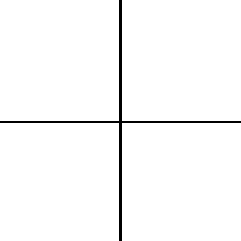
\includegraphics{page_12.pdf}
\end{minipage}\\[.25in]
\underline{\bf{Task 2}} \begin{minipage}[t]{5.5in}To show that $H$ is a subgroup we need to show, for one thing, that if $\alpha \in H$ so is $\alpha^{-1}$.  What is the inverse of $a+bi$?  Try this on $\alpha = \frac12+\frac12 i$.  What is $\alpha ^{-1}$?\\[1in]
Is $\alpha \in H$?  You need to compute $\sqrt{\frac14+\frac14}$.\\[1in]
Draw $\alpha$ and $\alpha^{-1}$ in your picture as vectors.  How are their angles related?  How do you multiply two complex numbers to show $\alpha\alpha^{-1} = 1$?
\end{minipage}\\[1in]
\underline{\bf{Task 3}} Give an $\alpha$ \underline{not} in $H$.\\[1in]
\underline{\bf{Task 4}} Do you now need to check closure?
%
%
%
\clearpage
%
%
%
{\large \bf WORKSHEET ON ORDER}\\[.25in]
\addcontentsline{toc}{subsection}{Order}
The order of an element $a$ of a group $G$ is the order of the cyclic subgroup $[a]$ generated by $a$ in $G$.  Equivalently, it is the \underline{smallest} positive integer $m$ so that $a^m=e$.\\[.25in]
\underline{\bf{Task 1}} \begin{minipage}[t]{6in}Let $G$ be a cyclic group of order 18 generated by $a$.  Then\\[.2in]
 $G=\{e,a,a^2,a^3,a^4,a^5,a^6,a^7,a^8,a^9,a^{10},a^{11},a^{12},a^{13},a^{14},a^{15},a^{16},a^{17}\}$.\\[.2in]Give the order of each element of $G$ by filling out the chart:\\[.2in]
\begin{tabular*}{12cm}{c|@{\hspace{.75cm}}c@{\hspace{.75cm}}c@{\hspace{.75cm}}c@{\hspace{.75cm}}c@{\hspace{.75cm}}c@{\hspace{.75cm}}c@{\hspace{.75cm}}c@{\hspace{.75cm}}c@{\hspace{.75cm}}c}
$x$&$e$&$a$&$a^2$&$a^3$&$a^4$&$a^5$&$a^6$&$a^7$&$a^8$\\
\hline\\[-.1in]
order $x$\\

\end{tabular*}\\[.75in]
\begin{tabular*}{13cm}{c|@{\hspace{.75cm}}c@{\hspace{.75cm}}c@{\hspace{.75cm}}c@{\hspace{.75cm}}c@{\hspace{.75cm}}c@{\hspace{.75cm}}c@{\hspace{.75cm}}c@{\hspace{.75cm}}c@{\hspace{.75cm}}c}
$x$&$a^9$&$a^{10}$&$a^{11}$&$a^{12}$&$a^{13}$&$a^{14}$&$a^{15}$&$a^{16}$&$a^{17}$\\
\hline\\[-.1in]
order $x$\\
\end{tabular*}
\end{minipage}\\[1in]
\underline{\bf{Task 2}} Repeat Task 1 with $G$ being a cyclic group of order 24.
%
%
%
\clearpage
%
%
%
{\large \bf WORKSHEET ON GROUP TABLES}\\[.25in]
\addcontentsline{toc}{subsection}{Group Tables}
Give as many reasons as you can why each of these tables cannot be group operation tables.  You can state a group axiom that fails, or appeal to some of our theorems and results.\\[.2in]
{\Large\begin{tabular*}{2.0in}{c|c@{\hspace{.75cm}}c@{\hspace{.75cm}}c@{\hspace{.75cm}}c@{\hspace{.75cm}}c}
&$a$&$b$&$c$&$d$&$e$\\
\hline
$a$&$c$&$e$&$a$&$b$&$d$\\[.1in]
$b$&$d$&$c$&$b$&$e$&$a$\\[.1in]
$c$&$a$&$b$&$c$&$d$&$e$\\[.1in]
$d$&$e$&$a$&$d$&$c$&$b$\\[.1in]
$e$&$b$&$d$&$e$&$a$&$c$
\end{tabular*}}\\[.5in]
{\Large\begin{tabular*}{2.0in}{c|c@{\hspace{.75cm}}c@{\hspace{.75cm}}c@{\hspace{.75cm}}c@{\hspace{.75cm}}c}
&$a$&$b$&$c$&$d$&$e$\\
\hline
$a$&$c$&$e$&$a$&$b$&$d$\\[.1in]
$b$&$d$&$a$&$b$&$e$&$c$\\[.1in]
$c$&$a$&$b$&$c$&$d$&$e$\\[.1in]
$d$&$e$&$c$&$d$&$a$&$b$\\[.1in]
$e$&$b$&$d$&$e$&$c$&$a$
\end{tabular*}}\\[.5in]
{\Large\begin{tabular*}{2.0in}{c|c@{\hspace{.75cm}}c@{\hspace{.75cm}}c@{\hspace{.75cm}}c@{\hspace{.75cm}}c}
&$a$&$b$&$c$&$d$&$e$\\
\hline
$a$&$e$&$d$&$b$&$c$&$a$\\[.1in]
$b$&$c$&$e$&$d$&$a$&$b$\\[.1in]
$c$&$d$&$a$&$e$&$b$&$c$\\[.1in]
$d$&$b$&$c$&$a$&$e$&$d$\\[.1in]
$e$&$a$&$b$&$c$&$d$&$e$
\end{tabular*}}%
%
%
\clearpage
%
%
%
{\large \bf WORKSHEET ON COMPLEX NUMBERS }\\[.25in]
\addcontentsline{toc}{subsection}{Complex Numbers }
\rule{0in}{.25in}
\underline{\bf{Task 1}} \begin{minipage}[t]{3in}$i^2 =$\\[.25in]
$(1+i)(2-3i)=$
\end{minipage}\\[.75in]
\underline{\bf{Task 2}} \begin{minipage}[t]{6in}Locate each of the following in the cartesian plane.\\[.25in]
(a) 1, $(-1+i\sqrt3)/2$, $(-1-i\sqrt3)/2$\\ \rule{4in}{0in}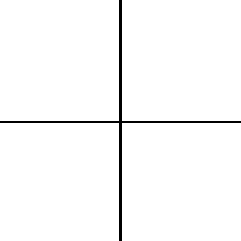
\includegraphics{page_12.pdf}\\
(b) 1, $-1$, $i$, $-i$\\ \rule{3in}{0in}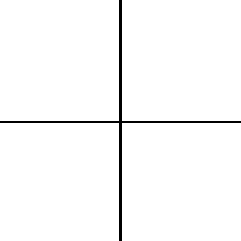
\includegraphics{page_12.pdf}\\
(c) \begin{minipage}[t]{5in}Connect each of the points in (a) and describe the properties of the figure.  Repeat with (b).\end{minipage}\\[1in]
(d) \begin{minipage}[t]{5in}What are the roots of $x^3-1=0$, $x^4-1=0$, and how is this question related to the above parts?\end{minipage}
\end{minipage}
%
\clearpage
%
\underline{\bf{Task 3}} If $r$ and $s$ are roots of $x^2-7x+43=0$, what are $r+s$ and $rs$?\\[1in]
\underline{\bf{Task 4}} \begin{minipage}[t]{6in}Use $(x-a)(x-b) = x^2-(a+b)x+ab$ to resolve Task 3.\\[1.25in]
Give a similar expression for $(x-a)(x-b)(x-c)$.\\[1in]
What is the sum of the roots of $x^3-3x^2+2x-14=0$?  The product of the roots?\\[1in]
Let 1, $r$, $s$ be roots of $x^3-1=0$.\\[.25in]
The product of the roots is $1rs=$\rule{1in}{.01in}, so that $rs=$\rule{1in}{,01in}.\\[.25in]
Also, $r^3=$\rule{1in}{.01in}, $s^3=$\rule{1in}{.01in}.\\[.25in]
Explain why $r^2=-r-1$ and \begin{minipage}[b]{.4in}$$r=\frac{1}{s}$$\end{minipage} and \begin{minipage}[b]{.55in}$$r^3=\frac{r^2}{s}$$\end{minipage}.\\[1in]
Why is $r^2=s$?
\end{minipage}
%
%
%
\clearpage
%
%
%
{\large \bf MULTIPLICATION TABLE OF ROOTS }\\[.25in]
\addcontentsline{toc}{subsection}{Table of Roots }
\underline{\bf{Task 1}} Use $x^n-1=(x-1)(x^{n-1}+x^{n-2}+\dots+x+1)$ to complete the chart:\\[.2in]
\fbox{
\begin{tabular}{c@{\hspace{1.5in}}c@{\hspace{1.5in}}c}
&{\bf FACTORS}&{\bf ROOTS}\\
\hline\\[-.15in]
$x^2-1=0$&$(x-1)(x+1)$&$1$,$-1$\\[.25in]
$x^3-1=0$&&\\[.25in]
$x^4-1=0$&&
\end{tabular}
}\\[.25in]
For convenience, you might want to label the roots of $x^3-1=0$ as $1$, $\beta$, $\gamma$.\\[.25in]
\underline{\bf{Task 2}} Make the multiplication table for each set of roots:\\[.2in]
\begin{tabular}{c|@{\hspace{.2in}}c@{\hspace{.2in}}c}
&1&$-1$\\
\hline\\[-.1in]
1\\[.2in]
$-1$
\end{tabular}\hfill
\begin{tabular}{c|@{\hspace{.2in}}c@{\hspace{.2in}}c@{\hspace{.2in}}c}
&1&$\beta$&$\gamma$\\
\hline\\[-.1in]
1\\[.2in]
$\beta$\\[.2in]
$\gamma$
\end{tabular}\hfill
\begin{tabular}{c|@{\hspace{.25in}}c@{\hspace{.25in}}c@{\hspace{.25in}}c@{\hspace{.25in}}c}
&\phantom{1}&\phantom{$\beta$}&\phantom{$\gamma$}&\phantom{xxx}\\
\hline\\[.1in]
\phantom{1}\\[.25in]
\phantom{$\beta$}\\[.25in]
\phantom{$\gamma$}
\end{tabular}\\[.5in]
\underline{\bf{Task 3}} Plot separately the set of roots for $x^2-1=0$, $x^3-1=0$, and $x^4-1=0$.\\[.2in]
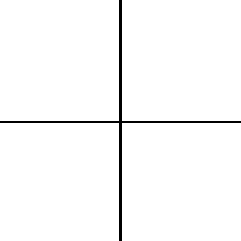
\includegraphics{page_12.pdf}\hfill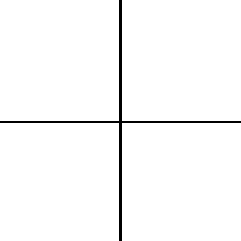
\includegraphics{page_12.pdf}\hfill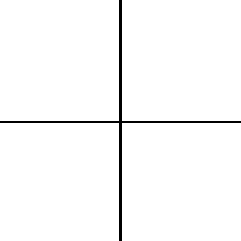
\includegraphics{page_12.pdf}\\[.2in]
Connect the points and describe the geometrical figure produced.\\[.2in]
\underline{\bf{Task 4}} Conjecture what happens for $x^5-1=0$, $x^6-1=0$.
%
%
%
\clearpage
%
%
%
{\large \bf GROUP TABLE FOR THE SIXTH ROOTS OF UNITY }\\[.25in]
\addcontentsline{toc}{subsection}{Sixth Roots of Unity }
The goal here is to find the six roots of $x^6-1=0$, plot them, and make their group table.\\[.25in]
\underline{\bf{Task 1}} \begin{minipage}[t]{6in}Factor $x^6-1=(x^3-1)(\hspace{.5in})=(\hspace{.5in})(\hspace{.75in})(\hspace{.5in})(\hspace{.75in})$\\[.2in]
The six roots are:\\[1in]
\end{minipage}\\
\underline{\bf{Task 2}}  Plot these six complex numbers.\\[.5in]
\raisebox{1in}{Connect them, forming a \rule{1.75in}{.01in}}\hfill  \begin{minipage}[t]{2in}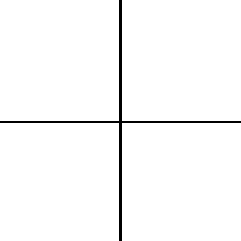
\includegraphics{page_12.pdf}\end{minipage}\\[.2in]
\underline{\bf{Task 3}} Label the six roots $1,\,r,\,s,\,-1,\,-r,\,-s$ where $1$, $r$, $s$ are the roots of $x^3-1=0$.  Show why the last three are negatives of the first three.  Show why $rs=1$, $r^2=s$, $s^2=r$.\\[1.5in]
\underline{\bf{Task 4}} Make the group table\\
\rule{3.5in}{0in}\begin{tabular}{c|c@{\hspace{.25in}}c@{\hspace{.25in}}c@{\hspace{.25in}}c@{\hspace{.25in}}c@{\hspace{.25in}}c}
& 1& $r$ & $s$ & $-1$ & $-r$ & $-s$\\
\hline\\[-.1in]
1\\[.1in]
$r$\\[.1in]
$s$\\[.1in]
$-1$\\[.1in]
$-r$\\[.1in]
$-s$
\end{tabular}
%
%
%
\clearpage
%
%
%
{\large \bf MULTIPLICATION TABLE FOR THE ROOTS \\OF $x^8-1=0$ }\\[.25in]
\addcontentsline{toc}{subsection}{Eighth Roots of Unity}
FACTOR: $x^8-1=(x^4-1)(x^4+1)$.  The roots of $x^4-1=0$ are \rule{1.75in}{.01in}\\[.2in]
$x^4+1=x^4+2x^2+1-2x^2=(x^2+1)^2-(\sqrt2\,x)^2=(x^2-\sqrt2\,x+1)(x^2+\sqrt2\,x+1)$\\[.2in]
The other roots are:\hspace{1.25in}\begin{tabular}{c@{\hspace{.75in}}c}
$\displaystyle r=\frac{1}{\sqrt2}+\frac{i}{\sqrt2}$&$\displaystyle -r=\frac{-1}{\sqrt2}-\frac{i}{\sqrt2}$\\[.2in]
$\displaystyle s=\frac{-1}{\sqrt2}+\frac{i}{\sqrt2}$&$\displaystyle -s=\frac{1}{\sqrt2}-\frac{i}{\sqrt2}$
\end{tabular}\\[.2in]
\begin{minipage}[t]{2.5in}
These eight roots are spread evenly around a unit circle $45^\circ$ apart.
\end{minipage}\hspace{1.5in}
\begin{minipage}[c]{2.5in}\input{page_19.pdf_tex}\end{minipage}\\[.2in]
\underline{\bf{Task 1}} Use the fact that when you multiply complex numbers you add their arguments to express each of the following in terms of $1$, $-1$, $i$, $-i$, $r$, $s$, $-r$, $-s$.\\
\begin{equation*}\begin{split}
r^2 &=\hspace{1.5in}ir&=\hspace{1.5in}s^2=\\[.25in]
rs &= \hspace{1.5in}is&= \hspace{1.5in}\phantom{s^2=}
\end{split}\end{equation*}\\[.2in]
\underline{\bf{Task 2}} Complete the multiplication table\\[.2in]
\begin{tabular}{c|@{\hspace{.3in}}c@{\hspace{.3in}}c@{\hspace{.3in}}c@{\hspace{.3in}}c@{\hspace{.3in}}c@{\hspace{.3in}}c@{\hspace{.3in}}c@{\hspace{.3in}}c}
& 1& $-1$&$i$&$-i$&$r$&$s$&$-r$&$-s$\\
\hline\\[-.1in]
1\\[.15in]
$-1$\\[.15in]
$i$\\[.15in]
$-i$\\[.15in]
$r$\\[.15in]
$s$\\[.15in]
$-r$\\[.15in]
$-s$
\end{tabular}
%
%
%
\clearpage
%
%
%
{\large \bf COMPOSITION OF FUNCTIONS}\\[.25in]
\addcontentsline{toc}{subsection}{Composition of Functions}
\begin{minipage}[t]{4in}\begin{tabular}{r@{=}l@{\hspace{1in}}r@{=}l}
Let \quad$\displaystyle f_1(x)$ & $\displaystyle x$ & $\displaystyle f_4(x)$ & $\displaystyle\frac{1}{x}$\\[.5in]
$\displaystyle f_2(x)$ & $\displaystyle\frac{1}{1-x}$ & $\displaystyle f_5(x)$ & $\displaystyle1-x$\\[.5in]
$\displaystyle f_3(x)$ & $\displaystyle\frac{x-1}{x}$ & $\displaystyle f_6(x)$ & $\displaystyle\frac{x}{x-1}$
\end{tabular}\end{minipage}\hfill\begin{minipage}[b]{2.25in} The following ``multiplication" table can be formed using composition of functions as the operation\end{minipage}\\[1in]
EXAMPLE: $f_2\;\circ\;f_6=f_5$ since {$\displaystyle f_2\left( \frac{x}{x-1}\right) = \frac{1}{1-\frac{x}{x-1}} = 1-x = f_5(x)$}\\[.25in]
\begin{tabular}{c|@{\hspace{.5in}}c@{\hspace{.5in}}c@{\hspace{.5in}}c@{\hspace{.5in}}c@{\hspace{.5in}}c@{\hspace{.5in}}c}
$\circ$ & $x$ & $\displaystyle\frac{1}{1-x}$ & $\displaystyle\frac{x-1}{x}$ & $\displaystyle\frac{1}{x}$ & $\displaystyle1-x$ & $\displaystyle\frac{x}{x-1}$ \\[.1in]
\hline \\[-.05in]
$\displaystyle f_1=x$ & $\displaystyle x$ & $\displaystyle\frac{1}{1-x}$ & $\displaystyle\frac{x-1}{x}$ & $\displaystyle\frac{1}{x}$ & $\displaystyle 1-x$ & $\displaystyle\frac{x}{x-1}$ \\[.5in]
$\displaystyle f_2=\frac{1}{1-x}$ & $\displaystyle\frac{1}{1-x}$ & $\displaystyle\frac{x-1}{x}$ & $\displaystyle x$ & $\displaystyle\frac{x}{x-1}$ & $\displaystyle\frac{1}{x}$ &$\displaystyle 1-x$ \\[.5in]
$\displaystyle f_3=\frac{x-1}{x}$ & $\displaystyle\frac{x-1}{x}$\\[.5in]
$\displaystyle f_4=\frac{1}{x}$ & $\displaystyle\frac{1}{x}$\\[.5in]
$\displaystyle f_5=1-x$ & $\displaystyle1-x$\\[.5in]
$\displaystyle f_6=\frac{x}{x-1}$ &$\displaystyle\frac{x}{x-1}$
\end{tabular}
%
%
%
\clearpage
%
%
%
{\large \bf COMPOSITION OF FUNCTIONS (CONT)}\\[.25in]
Rewrite the table using $f_1, f_2, f_3, f_4, f_5, f_6$\\[.25in]
\begin{tabular}{c|@{\hspace{.3in}}c@{\hspace{.3in}}c@{\hspace{.3in}}c@{\hspace{.3in}}c@{\hspace{.3in}}c@{\hspace{.3in}}c}
$\circ$ & $f_1$ & $f_2$ & $f_3$ & $f_4$ & $f_5$ & $f_6$\\
\hline\\
$f_1$ \\[.3in]
$f_2$ \\[.3in]
$f_3$ \\[.3in]
$f_4$ \\[.3in]
$f_5$ \\[.3in]
$f_6$
\end{tabular} \raisebox{1.3in}{\hspace{.75in} List properties of this table.}\\[.5in]
Complete the table showing inverses \hfill \begin{tabular}{c|@{\hspace{.25in}}c@{\hspace{.25in}}c@{\hspace{.25in}}c@{\hspace{.25in}}c@{\hspace{.25in}}c@{\hspace{.25in}}c}
$f$ & $f_1$ & $f_2$ & $f_3$ & $f_4$ & $f_5$ & $f_6$\\
\hline\\[-.1in]
$f^{-1}$
\end{tabular}\\[1in]
List all the subsets of $\{f_1, f_2,f_3, f_4,f_5,f_6\}$ that are closed under $\circ$.
%
%
%
\clearpage
%
%
%
{\large \bf EULER $\phi$-FUNCTION}\\[.25in]
\addcontentsline{toc}{subsection}{Euler $\phi$-Function}
$\phi(n)$ is the number of positive integers less than $n$ that are relatively prime to $n$.  Here is a partial table:\\[.1in]
\begin{tabular}{c|@{\hspace{.25in}}c@{\hspace{.25in}}c@{\hspace{.25in}}c@{\hspace{.25in}}c@{\hspace{.25in}}c@{\hspace{.25in}}c@{\hspace{.25in}}c@{\hspace{.25in}}c@{\hspace{.25in}}c@{\hspace{.25in}}c@{\hspace{.25in}}c@{\hspace{.25in}}c@{\hspace{.25in}}c@{\hspace{.25in}}c@{\hspace{.25in}}c@{\hspace{.25in}}c}
$n$ & 1 & 2 & 3 & 4& 5& 6 & 7 & 8 & 9 & 10 & 11 & 12 & 13 & 14 & 15 & 16\\
\hline\\[-.1in]
$\phi(n)$ & 1 & 1 & 2 & 2 & 4 & 2 & 6 & 4 & 6 & 4 & 10
\end{tabular}\\[.25in]
\underline{\bf{Task 1}} Complete the table.  Any conjectures?\vfill
\underline{\bf{Task 2}} Conjecture and prove a formula for $\phi(p)$, $p$ a prime.\vfill
\underline{\bf{Task 3}} Prove a formula for $\phi(p^2)$.\vfill
\underline{\bf{Task 4}} Compute $\phi(7^3)$ by listing the integers.\vfill
\underline{\bf{Task 5}} Prove a formula for $\phi(p^n)$.\vfill
\underline{\bf{Task 6}} Prove that $\phi(11^n)$ is a multiple of 10, for all $n$.\vfill
\underline{\bf{Task 7}} Show that $\phi(16)\cdot\phi(9) =  \phi(16\cdot 9)$\vfill
\clearpage
\underline{\bf{Task 8}} Find all $x$ such that $\phi(x)=n$ where:\\[.1in]
(a) $n$ =1 \hfill (b) $n$=2 \hfill (c) $n$=4 \hspace{2in} \vfill
\underline{\bf{Task 9}} \begin{minipage}[t]{6in}The notation $(a,b)=1$ means that $a$ and $b$ are relatively prime.\\
Prove that if $(a,m)=1$, then $(m-a,m)=1$.\end{minipage}\vfill
\underline{\bf{Task 10}} Prove that $\phi(n)$ is even for $n\geq 3$.\vfill
\underline{\bf{Task 11}} \begin{minipage}[t]{6in}It can be proved that if $(m,n)=1$, then $\phi(mn)=\phi(m)\phi(n)$.\\
Use this to compute $\phi(72)$; also compute $\phi(120)$.\end{minipage}\vfill
\underline{\bf{Task 12}} Prove that if $n=p_1^{e_1}p_2^{e_2}p_3^{e_3}$, then $\phi(n)=n\left(1-\frac{1}{p_1}\right)\left(1-\frac{1}{p_2}\right)\left(1-\frac{1}{p_3}\right)$.\vfill
%
%
%
\clearpage
%
%
%
{\large \bf WORKSHEET ON INVERTIBLES}\\[.25in]
\addcontentsline{toc}{subsection}{Invertibles}
Let $Z_m=\{\bar{0}$, $\bar{1}$, $\bar{2}$, $\bar{3}$, \dots, $\overline{m-1)}\}$ and $V_m$ be the set of invertibles of $Z_m$ consisting of those elements of $Z_m$ that have \textit{multiplicative} inverses.  For each $Z_m$ make a table of inverses of those elements that have multiplicative inverses and list $V_m$.  Here the ``bar" indicates an equivalence class.  $\bar{2}$ indicates the set of all integers in $Z$ whose remainder is 2 upon division by $m$.  Once understood, the ``bar'' is omitted.\\[.25in]
\underline{SAMPLE}:\\
\begin{tabular}{l@{\hspace{.5in}}l@{\hspace{.5in}}l}
$Z_3=\{0,1,2\}$ & \begin{tabular}{c|ccc}$x$&0&1&2\\ \hline\\[-.1in] $x^{-1}$ & & 1 & 2\end{tabular} & $V_3=\{1,2\}$\\[.75in]

$Z_4=\{0,1,2,3\}$ & \begin{tabular}{c|cccc}$x$&0&1&2&3\\ \hline\\[-.1in] $x^{-1}$ & &  & \end{tabular} & $V_4=\{\hspace{1in}\}$\\[.75in]
$Z_5=\{0,1,2,3,4\}$ & \begin{tabular}{c|ccccc}$x$&0&1&2&3&4\\ \hline\\[-.1in] $x^{-1}$ & &  & \end{tabular} & $V_5=\{\hspace{1in}\}$\\[.75in]
$Z_6=\{0,1,2,3,4,5\}$ & \begin{tabular}{c|cccccc}$x$&0&1&2&3&4&5\\ \hline\\[-.1in] $x^{-1}$ & &  & \end{tabular} & $V_6=\{\hspace{1in}\}$\\[.75in]
$Z_7=\{0,1,2,3,4,5,6\}$ & \begin{tabular}{c|ccccccc}$x$&0&1&2&3&4&5&6\\ \hline\\[-.1in] $x^{-1}$ & &  & \end{tabular} & $V_7=\{\hspace{1in}\}$\end{tabular}\\[.75in]
Can you conjecture which elements of $Z_{30}$ are invertibles?\vfill
How many invertibles does $Z_p$ have where $p$ is a prime?\vfill
How is the Euler $\phi$-function related to these questions?\vfill
%
%
%
\clearpage
%
%
%
{\large \bf PRESERVATION OF OPERATION}\\[.25in]
\addcontentsline{toc}{subsection}{Preservation of Operation}
In the following chart you are asked to verify whether certain familiar functions satisfy\\[.25in]
 $f(a\circ b)=f(a)\,\square\, f(b)$.  The operations $\circ$ and $\square$ can be addition or multiplication or a mixture.\\[.5in]
\begin{tabular}{l@{\hspace{.75in}}l@{\hspace{.75in}}l}
FUNCTION & YES OR NO & REASON\\
\hline\\[-.1in]
$f(x)=x^3$ & yes & $f(xy)=(xy)^3 = x^3y^3=f(x)f(y)$\\[.4in]
$f(x) = x^4$\\[.4in]
$f(x)=e^x$\\[.4in]
$f(x)=\displaystyle\frac32 x$\\[.4in]
$f(x)=2x+1$\\[.4in]
$f(x)=\ln x$\\[.4in]
$f(x)=|x|$\\[.4in]
$f(x)=\sqrt{x}$\\[.4in]
$f(x)=2x^3$\\[.4in]
$f(x)=\det x$\\[.4in]
$\theta(f) = f'$\\
(the derivative)
\end{tabular}
%
%
%
\clearpage
%
%
%
{\large \bf A SPECIAL ISOMORPHISM}\\[.25in]
\addcontentsline{toc}{subsection}{A Special Isomorphism}
\underline{\bf{Task 1}} Show that the mapping $\theta:G\rightarrow G$ given by $\theta(g)=g^{-1}$ is an isomorphism if $G$ is abelian.\\[.25in]
STEP 1 $\theta$ is 1-to-1.  To show this we need to show that if $\theta(g_1)=\theta(g_2)$ then\\[.25in]
\rule{4in}{.01in}.  Since $\theta(g_1)=\theta(g_2)$  we get \\[.25in]
\rule{4in}{.01in}.  Now by taking inverses, we obtain\\[.25in]
\rule{4in}{.01in}.\\[1in]
STEP 2  Show that $\theta$ is onto.\\[1in]
STEP 3  Show that $\theta$ preserves the operation\\[1in]
\underline{\bf{Task 2}}  Use $\theta(g)=g^{-1}$ to tabulate an isomorphism from $S_3$, the group of symmetries of an equilateral triangle, to itself.\\[.25in]
\begin{tabular*}{5in}{c|l}
$g$ &\\
\hline\\[-.1in]
$\theta(g)$
\end{tabular*} \\[.5in]
\underline{\bf{Task 3}} Show that the above result is false if $G$ is \underline{not} abelian.
%
%
%
\clearpage
%
%
%
{\large \bf 	MATCHING GROUPS}\\[.25in]
\addcontentsline{toc}{subsection}{Matching Groups}
There are two nonisomorphic groups of order 4, the cyclic group and the Klein 4-group whose elements $x$ satisfy $x^2=e$.\\[.25in]
For each of the following groups, label $A$ if it is isomorphic to the cyclic group and $B$ if it is isomorphic to the Klein group.\\[.25in]
\parbox{4in}{\rule{1in}{.01in} $[\;(1234)\;]$\\[.5in]
\rule{1in}{.01in} $[ -i]$\\[.5in]
\rule{1in}{.01in} $\{ e,a,a^2,a^3\}$\\[.5in]
\rule{1in}{.01in} $[i]$\\[.5in]
\rule{1in}{.01in} Rectangle Group\\[.5in]
\rule{1in}{.01in} $\{1,-1, i,-i\}$\\[.5in]
\rule{1in}{.01in} $\{0,1,2,3\}$ under addition mod 4\\[.5in]
\rule{1in}{.01in} $\{(1), (12), (34), (12)(34)\}$
}\raisebox{2.25in}{\fbox{\parbox{1in}{A. Cyclic\\B.  Klein}}}
%
%
%
\clearpage
%
%
%
{\large\bf WORKSHEET ON AN $8\times 8$ GROUP TABLE --  $Z_8$}\\[.25in]
\addcontentsline{toc}{subsection}{Groups of Order 8}
%
\textbf{\underline{Task 1}} Fill in the following table where each of the 64 entries is found by addition modulo 8; i.e. add the two numbers, divide by 8, and record the remainder.\\[.5in]
\rule{0 in}{.5in}
\begin{tabular}{c|@{\hspace{.2in}}c@{\hspace{.2in}}|@{\hspace{.2in}}c@{\hspace{.2in}}|@{\hspace{.2in}}c@{\hspace{.2in}}|@{\hspace{.2in}}c@{\hspace{.2in}}|@{\hspace{.2in}}c@{\hspace{.2in}}|@{\hspace{.2in}}c@{\hspace{.2in}}|@{\hspace{.2in}}c@{\hspace{.2in}}|@{\hspace{.2in}}c@{\hspace{.2in}}}
$\oplus$ & 0 & 1 & 2 & 3 & 4 & 5 & 6 & 7\\
\hline
\rule[-.15in]{.0in}{.4in}0&&&&&&&&\\
\hline
\rule[-.15in]{.0in}{.4in}1&&&&&&&&\\
\hline
\rule[-.15in]{.0in}{.4in}2&&&&&&&&\\
\hline
\rule[-.15in]{.0in}{.4in}3&&&&&&&&\\
\hline
\rule[-.15in]{.0in}{.4in}4&&&&&&&&\\
\hline
\rule[-.15in]{.0in}{.4in}5&&&&&&&&\\
\hline
\rule[-.15in]{.0in}{.4in}6&&&&&&&&\\
\hline
\rule[-.15in]{.0in}{.4in}7&&&&&&&&\\
\end{tabular}\\[.3in]
\textbf{MAKE A TABLE OF INVERSES\hfill \parbox{2in}{DRAW THE LATTICE OF SUBGROUPS.}}\\[.25in]
$\begin{array}{c|cccccccc}
&~0~&~1~&~2~&~3~&~4~&~5~&~6~&~7~\\
\hline
&
\end{array}$\\[.5in]
\textbf{LABEL AND LIST ALL THE\\ SUBGROUPS.}\vfill
%
%
%
\clearpage
%
%
%
{\large\bfseries WORKSHEET ON AN $8\times 8$ GROUP TABLE -- $Z_2 \times Z_4$}\\[.25in]

\textbf{\underline{Task 1}} Fill in the following table using bitwise addition mod 2 in the left-most slot and bitwise addition mod 4 in the right-most slot.\\[.5in]
\begin{tabular}{c|@{\hspace{.15in}}c@{\hspace{.15in}}|@{\hspace{.15in}}c@{\hspace{.15in}}|@{\hspace{.15in}}c@{\hspace{.15in}}|@{\hspace{.15in}}c@{\hspace{.15in}}|@{\hspace{.15in}}c@{\hspace{.15in}}|@{\hspace{.15in}}c@{\hspace{.15in}}|@{\hspace{.15in}}c@{\hspace{.15in}}|@{\hspace{.15in}}c@{\hspace{.15in}}}
$\oplus$ & 00 & 01 & 02 & 03 & 10 & 11 & 12 & 13\\
\hline
\rule[-.15in]{.0in}{.4in}00&&&&&&&&\\
\hline
\rule[-.15in]{.0in}{.4in}01&&&&&&&&\\
\hline
\rule[-.15in]{.0in}{.4in}02&&&&&&&&\\
\hline
\rule[-.15in]{.0in}{.4in}03&&&&&&&&\\
\hline
\rule[-.15in]{.0in}{.4in}10&&&&&&&&\\
\hline
\rule[-.15in]{.0in}{.4in}11&&&&&&&&\\
\hline
\rule[-.15in]{.0in}{.4in}12&&&&&&&&\\
\hline
\rule[-.15in]{.0in}{.4in}13&&&&&&&&\\
\end{tabular}\\[.3in]
\textbf{MAKE A TABLE OF INVERSES\hfill \parbox{2in}{DRAW THE LATTICE OF SUBGROUPS.}}\\[.25in]
$\begin{array}{c|cccccccc}
\phantom{\oplus}&\phantom{00}&\phantom{01}&\phantom{02}&\phantom{03}&\phantom{10}&\phantom{11}&\phantom{12}&\phantom{13}\\
\hline
\phantom{00}\\
\end{array}$\\[.5in]
\textbf{LABEL AND LIST ALL THE\\ SUBGROUPS.}\vfill
%
%
%
\clearpage
%
%
%
{\large\bfseries WORKSHEET ON AN $8\times 8$ GROUP TABLE -- $Z_2 \times Z_2 \times Z_2$}\\[.25in]

\textbf{\underline{Task 1}} Fill in the following table using \underline{bitwise addition mod 2}.\\[.5in]
\begin{tabular}{c|@{\hspace{.1in}}c@{\hspace{.1in}}|@{\hspace{.1in}}c@{\hspace{.1in}}|@{\hspace{.1in}}c@{\hspace{.1in}}|@{\hspace{.1in}}c@{\hspace{.1in}}|@{\hspace{.1in}}c@{\hspace{.1in}}|@{\hspace{.1in}}c@{\hspace{.1in}}|@{\hspace{.1in}}c@{\hspace{.1in}}|@{\hspace{.1in}}c@{\hspace{.1in}}}
$\oplus$ & 000 & 001 & 010 & 011 & 100 & 101 & 110 & 111\\
\hline
\rule[-.15in]{.0in}{.4in}000&&&&&&&&\\
\hline
\rule[-.15in]{.0in}{.4in}001&&&&&&&&\\
\hline
\rule[-.15in]{.0in}{.4in}010&&&&&&&&\\
\hline
\rule[-.15in]{.0in}{.4in}011&&&&&&&&\\
\hline
\rule[-.15in]{.0in}{.4in}100&&&&&&&&\\
\hline
\rule[-.15in]{.0in}{.4in}101&&&&&&&&\\
\hline
\rule[-.15in]{.0in}{.4in}110&&&&&&&&\\
\hline
\rule[-.15in]{.0in}{.4in}111&&&&&&&&\\
\end{tabular}\\[.3in]
\textbf{MAKE A TABLE OF INVERSES\hfill \parbox{2in}{DRAW THE LATTICE OF SUBGROUPS.}}\\[.25in]
$\begin{array}{c|cccccccc}
\phantom{\oplus}&\phantom{00}&\phantom{01}&\phantom{02}&\phantom{03}&\phantom{10}&\phantom{11}&\phantom{12}&\phantom{13}\\
\hline
\phantom{00}\\
\end{array}$\\[.5in]
\textbf{LABEL AND LIST ALL THE\\ SUBGROUPS.}\vfill
%
%
%
\clearpage
%
%
%
{\large\bfseries WORKSHEET ON AN $8\times 8$ GROUP TABLE --\\ THE QUATERNIONS}\\[.25in]
\textbf{\underline{Task 1}} Fill in the following table using the operations:
$$i^2=j^2=k^2=-1, \;ij=-ji=k,\; jk=-kj=i,\; ki=-ik=j$$
\def\svgwidth{.75in}
\centerline{\input{drawing.pdf_tex}}\\[.2in]
\begin{tabular}{c|@{\hspace{.2in}}c@{\hspace{.2in}}|@{\hspace{.15in}}c@{\hspace{.15in}}|@{\hspace{.2in}}c@{\hspace{.2in}}|@{\hspace{.15in}}c@{\hspace{.15in}}|@{\hspace{.2in}}c@{\hspace{.2in}}|@{\hspace{.15in}}c@{\hspace{.15in}}|@{\hspace{.2in}}c@{\hspace{.2in}}|@{\hspace{.15in}}c@{\hspace{.15in}}}
$\otimes$ & 1 & $-1$ & $i$ & $-i$ & $j$ & $-j$ & $k$ & $-k$\\
\hline
\rule[-.15in]{.0in}{.4in}$1$&&&&&&&&\\
\hline
\rule[-.15in]{.0in}{.4in}$-1$&&&&&&&&\\
\hline
\rule[-.15in]{.0in}{.4in}$i$&&&&&&&&\\
\hline
\rule[-.15in]{.0in}{.4in}$-i$&&&&&&&&\\
\hline
\rule[-.15in]{.0in}{.4in}$j$&&&&&&&&\\
\hline
\rule[-.15in]{.0in}{.4in}$-j$&&&&&&&&\\
\hline
\rule[-.15in]{.0in}{.4in}$k$&&&&&&&&\\
\hline
\rule[-.15in]{.0in}{.4in}$-k$&&&&&&&&\\
\end{tabular}\\[.3in]
\textbf{MAKE A TABLE OF INVERSES\hfill \parbox{2in}{DRAW THE LATTICE OF SUBGROUPS.}}\\[.25in]
$\begin{array}{c|cccccccc}
\phantom{\oplus}&\phantom{00}&\phantom{01}&\phantom{02}&\phantom{03}&\phantom{10}&\phantom{11}&\phantom{12}&\phantom{13}\\
\hline
\phantom{00}\\
\end{array}$\\[.5in]
\textbf{LABEL AND LIST ALL THE\\ SUBGROUPS.}\vfill
%
%
%
\clearpage
%
%
%
{\large\bfseries WORKSHEET ON AN $8\times 8$ GROUP TABLE -- THE OCTIC GROUP}\\[.25in]
\textbf{\underline{Task 1}} Fill in the following table using $fr=r^3f$.  These eight elements are the eight symmetries of a square.\\[.5in]
\begin{tabular}{c|@{\hspace{.2in}}c@{\hspace{.2in}}|@{\hspace{.2in}}c@{\hspace{.2in}}|@{\hspace{.2in}}c@{\hspace{.2in}}|@{\hspace{.2in}}c@{\hspace{.2in}}|@{\hspace{.2in}}c@{\hspace{.2in}}|@{\hspace{.2in}}c@{\hspace{.2in}}|@{\hspace{.2in}}c@{\hspace{.2in}}|@{\hspace{.2in}}c@{\hspace{.2in}}}
$\square$ & 1 & $r$ & $r^2$ & $r^3$ & $f$ & $rf$ & $r^2f$ & $r^3f$\\
\hline
\rule[-.15in]{.0in}{.4in}$1$&&&&&&&&\\
\hline
\rule[-.15in]{.0in}{.4in}$r$&&&&&&&&\\
\hline
\rule[-.15in]{.0in}{.4in}$r^2$&&&&&&&&\\
\hline
\rule[-.15in]{.0in}{.4in}$r^3$&&&&&&&&\\
\hline
\rule[-.15in]{.0in}{.4in}$f$&&&&&&&&\\
\hline
\rule[-.15in]{.0in}{.4in}$rf$&&&&&&&&\\
\hline
\rule[-.15in]{.0in}{.4in}$r^2f$&&&&&&&&\\
\hline
\rule[-.15in]{.0in}{.4in}$r^3f$&&&&&&&&\\
\end{tabular}\\[.3in]
\textbf{MAKE A TABLE OF INVERSES\hfill \parbox{2in}{DRAW THE LATTICE OF SUBGROUPS.}}\\[.25in]
$\begin{array}{c|cccccccc}
\phantom{\oplus}&\phantom{00}&\phantom{01}&\phantom{02}&\phantom{03}&\phantom{10}&\phantom{11}&\phantom{12}&\phantom{13}\\
\hline
\phantom{00}\\
\end{array}$\\[.5in]
\textbf{LABEL AND LIST ALL THE\\ SUBGROUPS.}\vfill
%
%
%
\clearpage
%
%
%
{\large \bf 	FIVE NONISOMORPHIC GROUPS OF ORDER 8}\\[.25in]
\addcontentsline{toc}{subsection}{Five Groups of Order 8 }
Listed next are the elements of these five groups along with their names.  You are asked to show why certain pairs are \underline{not} isomorphic.\\[.2in]
\begin{tabular}{ll}
CYCLIC & $\{e, a, a^2, a^3, a^4, a^5, a^6,a^7\}$\\[.5in]
QUATERNIONS & $\{ 1, -1, i, -i, j, -j, k, -k\}$\\[.5in]
OCTIC & $\{ (1), \rho, \rho^2, \rho^3,\phi,\rho\phi,\rho^2\phi,\rho^3\phi\}$\\[.5in]
\parbox{1.5in}{BIT STRINGS\\or $Z_2\times Z_2\times Z_2$} & $\{000, 001,010,011,100,101,110,111\}$\\[.5in]
$Z_2\times Z_4$ & $\{00,01,02,03,10,11,12,13\}$
\end{tabular}\\[.5in]
\underline{\bf{Task 1}} Give two reasons why the QUATERNIONS are \underline{not} isomorphic to the OCTIC group.\\ \vfill
\underline{\bf{Task 2}} Why is $Z_2 \times Z_4$ not isomorphic to $Z_2\times Z_2\times Z_2$?\\ \vfill
\underline{\bf{Task 3}} Why is the CYCLIC group not isomorphic to any of the other four?\vfill
%
%
%
\clearpage
%
%
%
{\large \bf 	WORKSHEET ON GROUP TABLES, ISOMORPHISMS}\\[.25in]
\addcontentsline{toc}{subsection}{Group Tables, Isomorphisms  }
Complete the following table using $\circ$ to mean composition of functions.  For example.
$$f_2\circ f_3 = f_2(f_3(x))=f_2(1-x)=\frac{1}{1-x}=f_4$$\\[.25in]
The six functions are:
$$f_1(x)=x\quad f_2(x)=\frac{1}{x}\quad f_3(x)=1-x\quad f_4(x)=\frac{1}{1-x}\quad f_5(x)=\frac{x-1}{x}\quad f_6=\frac{x}{x-1} $$\\[.25in]
\begin{tabular}{c|@{\hspace{.25in}}c@{\hspace{.5in}}c@{\hspace{.5in}}c@{\hspace{.5in}}c@{\hspace{.5in}}c@{\hspace{.5in}}c}
$\circ$ & $f_1$ & $f_2$ & $f_3$ & $f_4$ & $f_5$ & $f_6$\\
\hline\\[-.1in]
$f_1$ \\[.25in]
$f_2$\\[.25in]
$f_3$\\[.25in]
$f_4$\\[.25in]
$f_5$\\[.25in]
$f_6$\\
\end{tabular}\\[.75in]
Display an isomorphism between this group and either $S_3$ or $Z_6$.
%
%
%
\clearpage
%
%
%
{\large \bf 	FUNDAMENTAL THEOREM OF FINITE ABELIAN GROUPS}\\[.25in]%
\addcontentsline{toc}{subsection}{Fundamental Theorem} %
\underline{THEOREM:} \parbox[t]{5in}{Every finite abelian group can be written as a product of cyclic groups of prime power order.}\\[.25in]
\rule{.06in}{0in}\underline{EXAMPLES:} \parbox[t]{5in}{The Klein 4--Group is $Z_2\times Z_2$; the cyclic group of order 4 is $Z_4$.  The abelian group of order 6 is $Z_6$ which is isomorphic to the direct product $Z_2 \times Z_3$.}\\[.25in]
Let $G=\{1, 8, 12, 14, 18, 21, 27, 31, 34, 38, 44, 47, 51, 53, 57, 64\}$ be a group of order 16 under multiplication mod 65.  $G$ is isomorphic to one of:\\[.25in]
\parbox{3in}{\rule{.5in}{0in}$Z_{16}$\\
\rule{.35in}{0in}$Z_2 \times Z_8$\\
\rule{.35in}{0in}$Z_4 \times Z_4$\\
\rule{.2in}{0in}$Z_2 \times Z_2 \times Z_4$\\
$Z_2 \times Z_2 \times Z_2 \times Z_2$}%
\parbox{3in}{BUT WHICH ONE?\\[.25in] LOOK AT ORDERS!}\\[.25in]
\begin{tabular}{l|ccccccccccccccccc}
$x$ & 1 & 8 & 12 & 14 & 18 & 21 & 27 & 31 & 34 & 38 & 44 & 47 & 51 & 53 & 57 & 64\\
\hline\\[-.1in]
order $x$ & 1 & 4 & 4 & 2 & & 4 & 4 & & & 4& 4 & 4 & & 4 & 4&
\end{tabular}\\[.25in]
\underline{\bf{Task 1}} Why is $G$ not $Z_{16}$?\vfill
\underline{\bf{Task 2}} Why is $G$ not $Z_2 \times Z_8$?\vfill
\underline{\bf{Task 3}} What are the orders of elements in $Z_2\times Z_2\times Z_2\times Z_2$?\vfill
\underline{\bf{Task 4}} Which one must $G$ be?\vfill
%
%
\clearpage
%
%
\underline{\bf{Task 5}} $G =\{1, 9, 16, 22, 29, 53, 74, 79, 81\}$ is a  group of order 9 under multiplication modulo\\[.2in] 91.  Is $G$ isomorphic to $Z_9$ or $Z_3 \times Z_3$?  Why are these the only two possibilities?\\[.2in]
Make the table of orders and inverses.\\[.25in]
\begin{tabular}{l|c@{\hspace{.5in}}c@{\hspace{.5in}}c@{\hspace{.5in}}c@{\hspace{.5in}}c@{\hspace{.5in}}c@{\hspace{.5in}}c@{\hspace{.5in}}c@{\hspace{.5in}}c}
$x$ & 1 & 9 & 16 & 22 & 29 & 53 & 74 & 79 & 81\\
\hline\\[-.1in]
Order $x$ &
\end{tabular}\\[1in]
\begin{tabular}{l|c@{\hspace{.5in}}c@{\hspace{.5in}}c@{\hspace{.5in}}c@{\hspace{.5in}}c@{\hspace{.5in}}c@{\hspace{.5in}}c@{\hspace{.5in}}c@{\hspace{.5in}}c}
$x$ & 1 & 9 & 16 & 22 & 29 & 53 & 74 & 79 & 81\\
\hline\\[-.1in]
 $x^{-1}$\rule{.320in}{0in} &
\end{tabular}\\[1in]
\underline{\bf{Task 6}} \parbox[t]{6in}{ Identify all abelian groups (up to isomorphism) of order 360 by doing the following:\\[.2in]
A.  Express 360 as a product of prime numbers\\[1in]
B.  List the six direct product possibilities}
%
%
%
\clearpage
%
%
%
{\large \bf 	WHICH DIRECT PRODUCT?}\\[.25in]
\addcontentsline{toc}{subsection}{Which Direct Product}
$V_{45}=\{1, 2, 4, 7, 8, 11, 13, 14, 16, 17, 19, 22, 23, 26, 28, 29, 31, 32, 34, 37, 38, 41, 43, 44\}$ is a multiplicative group, using mod 45, of order 24. According to the fundamental theorem of finite abelian groups, $V_{45}$ is isomorphic to a direct product of cyclic groups, each having prime power order. The possibilities are:
$$ Z_3 \times Z_8 \qquad Z_2 \times Z_3 \times Z_4 \qquad Z_2\times Z_2\times Z_2 \times Z_3 $$
You do not include $Z_{24}$, $Z_6 \times Z_4$ or $Z_2 \times Z_{12}$ since the orders are not prime power.  Also notice that the cyclic group $Z_{24}$ is, in fact, $Z_3 \times Z_8$ which has (1, 1) as a generator.\\[.25in]
One way of determining which of these three is isomorphic to $V_{45}$ is by computing the orders of each element in $V_{45}$ and comparing with orders of elements in the direct products. By hand, this is not an easy feat.\\
\centerline{\fbox{\parbox{1.4in}{USING THE TI-92}}}
Clear home screen -- F1, 8\\
Clear input line -- CLEAR\\
Type in\\ \rule{.5in}{0in} \textit{Define} $f(n)=$ mod($22^n$, 45)\\
to determine the order of 22, eg., and enter.\\
Go to APPS and 6: Data/matrix editor, current and enter\\
If necessary clear columns with F6, 5.\\
Highlight C1 and enter.  Generate the sequence 1, 2, $\dots$, 24 with\\
 \rule{.5in}{0in}C1 = seq($n$, $n$, 1, 24) and enter.\\
Highlight C2 and generate $f(n)$ with\\
 \rule{.5in}{0in}C2 = seq($f(n)$, $n$, 1, 24) and enter.\\[.25in]
Column C2 will give $22^n$ reduced modulo 45 for $n$ ranging from 1 to 24.  You should find that $22^{12}\equiv 1$.\\
Now, if you return to the home screen [$2^\text{nd}$, QUIT] and just change the 22 to 2 we can quickly see, returning to APPS, 6, in column 2 that the order of 2 is 12.  Repeat this and complete the following table of orders.\\[.25in]
\begin{tabular}{c|c@{\hspace{.25in}}c@{\hspace{.25in}}c@{\hspace{.25in}}c@{\hspace{.25in}}c@{\hspace{.25in}}c@{\hspace{.25in}}c@{\hspace{.25in}}c@{\hspace{.25in}}c@{\hspace{.25in}}c@{\hspace{.25in}}c@{\hspace{.25in}}c}
$x$ &1 & 2 & 4 & 7 & 8 & 11 & 13 & 14 & 16 & 17 & 19 & 22\\
\hline\\[-.1in]
order $x$ & 1 & 12 & 6 & 12
\end{tabular}\\[.25in]
\begin{tabular}{c|c@{\hspace{.25in}}c@{\hspace{.25in}}c@{\hspace{.25in}}c@{\hspace{.25in}}c@{\hspace{.25in}}c@{\hspace{.25in}}c@{\hspace{.25in}}c@{\hspace{.25in}}c@{\hspace{.25in}}c@{\hspace{.25in}}c@{\hspace{.25in}}c}
$x$ & 23 & 26 & 28 & 29 & 31 & 32 & 34 & 37 & 38 & 41 & 43 & 44\\
\hline\\[-.1in]
order $x$ & &&&&&&&&&& 12 & 2
\end{tabular}
%
%
%
\clearpage
%
%
%
{\large \bf 	RINGS THAT ARE NOT INTEGRAL DOMAINS}\\[.25in]
\addcontentsline{toc}{subsection}{Rings, But Not I.D.}
A commutative ring $D$ with unity 1, having no zero-divisors is called an integral domain.\\[.25in]
\underline{\bf{Task 1}} Explain why $Z_{10}$ is not an integral domain.\\ \vfill
\underline{\bf{Task 2}} Why is $Z_{12}$ not?\\ \vfill
\underline{\bf{Task 3}} For which $m$ is $Z_m$ not an integral domain?\\ \vfill
\underline{\bf{Task 4}} Is $Z_2 \times Z_2$ an integral domain?\\ \vfill
\underline{\bf{Task 5}} Let $A$ and $B$ be integral domains.  Is $A\times B$ an integral domain?\\ \vfill
\underline{\bf{Task 6}} Is the set of all $2\times 2$ matrices with real entries with the usual addition an multiplication of matrices an integral domain?\\ \vfill
%
%
%
\clearpage
%
%
%
{\large \bf 	WORKSHEET ON POLYNOMIALS IN $Z_n[x]$}\\[.25in]
\addcontentsline{toc}{subsection}{Polynomials in $Z_n[x]$}
\underline{\bf{Task 1}} Tabulate each of $(x+\bar{2})(x+\bar{5})$ and $x(x+\bar{7})$ in $Z_{10}$ and thus show that they are equal.\\[.25in]
\begin{tabular}{c|@{\hspace{.4in}}c@{\hspace{.4in}}c@{\hspace{.4in}}c@{\hspace{.4in}}c@{\hspace{.4in}}c@{\hspace{.4in}}c@{\hspace{.4in}}c@{\hspace{.4in}}c@{\hspace{.4in}}c@{\hspace{.4in}}c}
$x$ & 0 & 1 & 2 & 3 & 4 & 5 & 6 & 7 & 8 & 9\\
\hline \\
$(x+\bar2)(x+\bar5)$ & & & 8\\[.2in]
\hline\\
$x(x+\bar7)$ &&& 8\\[.2in]
\end{tabular} \\[1in]
\underline{\bf{Task 2}} Show that $(x+\bar{3})(x+\bar{5}) = x(x+\bar{8})$ in $Z_{15}[x]$.\\ \vfill
\underline{\bf{Task 3}} Show that $(x+\bar{6})^2 = x^2$ in $Z_{12}[x]$.\\ \vfill
\underline{\bf{Task 4}} \parbox[t]{5in}{Our experience leads us to expect that deg $\alpha\beta$ = deg $\alpha$ + deg $\beta$\\[.2in] for polynomials $\alpha$ and $\beta$.\\[.2in]
But ... Show that $(\bar{2}x+\bar{1})(\bar{3}x+\bar{5})=x+\bar{5}$ in $Z_6[x]$.}\\ \vfill
%
%
\clearpage%
%
%
\underline{\bf{Task 5}} \parbox[t]{5in}{Show that in $Z_6[x]$\\[.2in]
$(\bar{2}x+\bar{5})(\bar{3}x+\bar{2}) = (x+\bar{4})$\\[1.25in]
$(\bar{3}x+\bar{3})(\bar{4}x^2+\bar{2}) = \bar{0}$\\[1.25in]}\\
\underline{\bf{Task 6}} \parbox[t]{5.5in}{In $Z_5[x], (\bar{2}x+\bar{1})(\bar{4}x+\bar{3})=(x+\bar{3})(\bar{3}x+\bar{1})$\\[1.5in]
Make these linear factors monic (leading coefficient is $\bar{1}$) by factoring out $\bar 2, \bar 4$,\\[.2in] and $\bar 3$.  For example $(\bar2 x+\bar 1)=\bar 2(x+\bar 3)$.  Then both sides become\\[.25in]
\rule{1.75in}{.01in}.}
%
%
%
\clearpage
%
%
%
{\large \bf 	WORKSHEET ON ANOTHER RING}\\[.25in]
\addcontentsline{toc}{subsection}{Another Ring}
Define``addition'' and ``multiplication'' as follows:
$$ a\oplus b = a+b-1 $$
$$ a\otimes b = a+b-ab$$
show that $(Z,\oplus, \otimes)$ is a ring by doing the following:\\[.25in]
\underline{\bf{Task 1}} Determine the ``0'', the additive identity.  Is there a unity?\\ \vfill
\underline{\bf{Task 2}} What is the additive inverse of $a$?  Why?\\ \vfill
\underline{\bf{Task 3}} Is $\oplus$ associative?  Is $\otimes$ associative?\\ \vfill
\underline{\bf{Task 4}} Show that $\otimes$ is distributive over $\oplus$.\\ \vfill
%
%
%
\clearpage
%
%
%
{\large \bf 	SUMMARY OF RINGS AND THEIR PROPERTIES}\\[.25in]
\addcontentsline{toc}{subsection}{Summary of Rings}
\begin{tabular}{l|c|c|l|l|l}
Ring & Form of Element & Unity & Abelian & Integral Domain & Field\\
\hline
&&&&\\[-.1in]
$Z$ & $k$ & 1 & Yes & Yes & No\\[.5in]
$Z_n$, $n$ composite &&&&\\[.5in]
$Z_p$, $p$ prime &&&&\\[.5in]
$Z[x]$ &&&&\\[.5in]
$nZ, \; n>1$ &&&&\\[.5in]
$M(Z)$, 2$\times$2 matrices &&&&\\[.5in]
$Z[i]$ &&&&\\[.5in]
$Z_3[i]$ &&&&\\[.5in]
$Z_2[i]$ &&&&\\[.5in]
$Z[\sqrt{2}] $&&&&\\[.5in]
$Q[\sqrt{2}]$ & $a+b\sqrt{2}$ &&&\\[.5in]
$Z\oplus Z$ &&&&
\end{tabular}
%
%
%
\clearpage
%
%
%
{\large \bf 	$Z_3[i]$ IS A FIELD WITH 9 ELEMENTS}\\[.25in]
\addcontentsline{toc}{subsection}{A Field With 9 Elements}
This field consists of all elements of the form $m+ni$ where $m$ and $n$ are in \{0,1,2\}.  The multiplication table is:\\[.25in]
\begin{tabular}{c|@{\hspace{.3in}}c@{\hspace{.3in}}c@{\hspace{.3in}}c@{\hspace{.3in}}c@{\hspace{.3in}}c@{\hspace{.3in}}c@{\hspace{.3in}}c@{\hspace{.3in}}c}
& 1 & 2 & $i$ & $1+i$ & $2+i$ & $2i$ & $1+2i$ & $2+2i$ \\
\hline\\[-.1in]
1 & 1 & 2 & $i$ & $1+i$ & $2+i$ & $2i$ & $1+2i$ & $2+2i$ \\[.3in]
2 & 2& 1 & $2i$ & $2+2i$ & $1+2i$ & $i$ & $2+i$ & $1+i$\\[.3in]
$i$ & $i$ & $2i$\\[.3in]
$1+i$ &$1+i$ & $2+2i$\\[.3in]
$2+i$ & $2+i$ & $1+2i$\\[.3in]
$2i$ & $2i$ & $i$\\[.3in]
$1+2i$ & $1+2i$ & $2+i$\\[.3in]
$2+2i$ & $2+2i$ & $1+i$
\end{tabular}\\[.2in]
\underline{\bf{Task 1}} Complete the table of inverses and orders:\\[.2in]
\begin{tabular}{c|@{\hspace{.4in}}c@{\hspace{.4in}}c@{\hspace{.4in}}c@{\hspace{.4in}}c@{\hspace{.4in}}c@{\hspace{.4in}}c@{\hspace{.4in}}c@{\hspace{.4in}}c}
$x$ & 1 & 2 & $i$ & $1+i$ & $2+i$ & $2i$ & $1+2i$ & $2+2i$ \\
\hline\\[-.1in]
$x^{-1}$ &\\[.1in]
\hline\\[-.1in]
order of $x$ &
\end{tabular}\\ \vfill
\underline{\bf{Task 2}} Which familiar group is the multiplicative group isomorphic to?\\ \vfill
%
%
%
\clearpage
%
%
%
{\large \bf 	APPLICATION OF A FAMOUS THEOREM}\\[.25in]
\addcontentsline{toc}{subsection}{Application of a Famous Theorem}
\underline{PROBLEM:} \parbox[t]{5.5in}{Explain why $x^7 -x = x(x-1)(x-2)(x-3)(x-4)(x-5)(x-6)$ in $Z_7[x]$.\\[.25in]
There are a number of ways of approaching this problem, several motivated by a similar question you couild ask in the $8^\text{th}$ grade.  Explain why $x^2-5x+6=(x-2)(x-3)$.  The following tasks guide you through three solutions.}\\[.25in]
\underline{\bf{Task 1}} Use a calculator and show that each of 1, 2, 3, 4, 5, 6 satisfies $x^7-x=0$; then use the factor theorem.\\ \vfill
\underline{\bf{Task 2}} Simplify the right hand side algebraically using $x-6=x+1,\, x-5=x+2,\,\\ x-4=x+3$.\\ \vfill
\underline{\bf{Task 3}} What famous Theorem has $x^7-x\equiv 0$ or $x^7\equiv x$ in it?\\ \vfill
\end{document}
